\documentclass{standalone}
\usepackage{tikz}
\usetikzlibrary{patterns, positioning}


\begin{document}
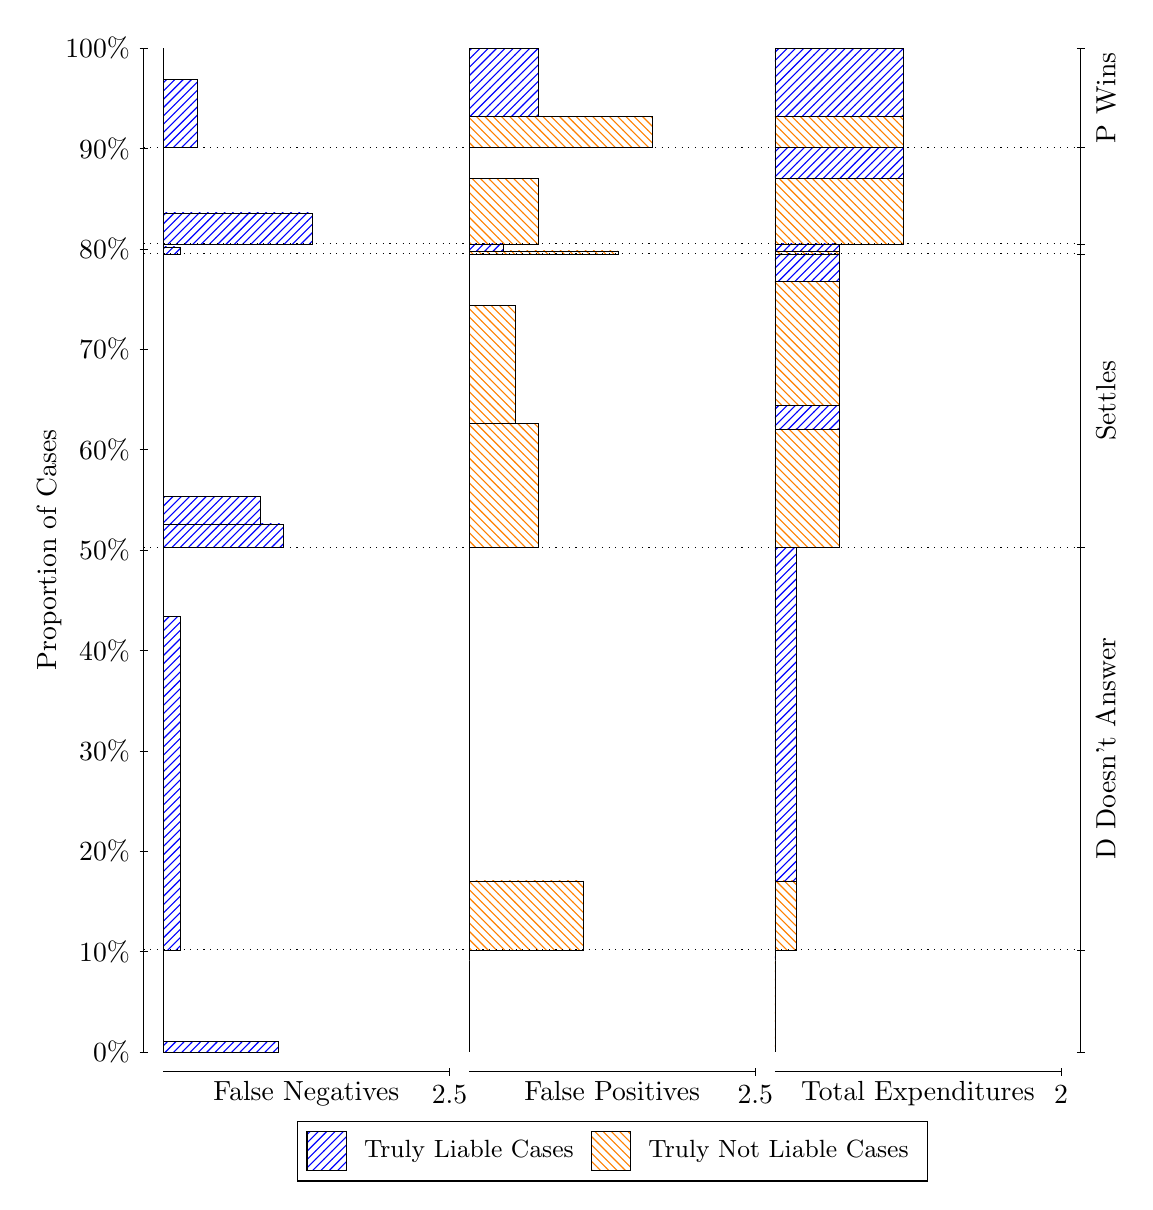
\begin{tikzpicture}
\draw[black, very thin] (1.5,1.75) -- (1.5,14.5);
\node[rotate=90, text=black, anchor=center] at (0.3, 8.125) {Proportion of Cases};
\draw[black, very thin] (1.45,1.75) -- (1.55,1.75);
\node[text=black, anchor=east] at (1.45, 1.75) {0\%};
\draw[black, very thin] (1.45,3.025) -- (1.55,3.025);
\node[text=black, anchor=east] at (1.45, 3.025) {10\%};
\draw[black, very thin] (1.45,4.3) -- (1.55,4.3);
\node[text=black, anchor=east] at (1.45, 4.3) {20\%};
\draw[black, very thin] (1.45,5.575) -- (1.55,5.575);
\node[text=black, anchor=east] at (1.45, 5.575) {30\%};
\draw[black, very thin] (1.45,6.85) -- (1.55,6.85);
\node[text=black, anchor=east] at (1.45, 6.85) {40\%};
\draw[black, very thin] (1.45,8.125) -- (1.55,8.125);
\node[text=black, anchor=east] at (1.45, 8.125) {50\%};
\draw[black, very thin] (1.45,9.4) -- (1.55,9.4);
\node[text=black, anchor=east] at (1.45, 9.4) {60\%};
\draw[black, very thin] (1.45,10.675) -- (1.55,10.675);
\node[text=black, anchor=east] at (1.45, 10.675) {70\%};
\draw[black, very thin] (1.45,11.95) -- (1.55,11.95);
\node[text=black, anchor=east] at (1.45, 11.95) {80\%};
\draw[black, very thin] (1.45,13.225) -- (1.55,13.225);
\node[text=black, anchor=east] at (1.45, 13.225) {90\%};
\draw[black, very thin] (1.45,14.5) -- (1.55,14.5);
\node[text=black, anchor=east] at (1.45, 14.5) {100\%};

\draw[black, very thin] (13.4,1.75) -- (13.4,14.5);
\draw[black, very thin] (13.35,1.75) -- (13.45,1.75);
\node[anchor=west] at (13.35, 1.75) {};
\draw[black, very thin] (13.35,3.0468) -- (13.45,3.0468);
\node[anchor=west] at (13.35, 3.0468) {};
\draw[black, very thin] (13.35,8.1578) -- (13.45,8.1578);
\node[anchor=west] at (13.35, 8.1578) {};
\draw[black, very thin] (13.35,11.886) -- (13.45,11.886);
\node[anchor=west] at (13.35, 11.886) {};
\draw[black, very thin] (13.35,12.012) -- (13.45,12.012);
\node[anchor=west] at (13.35, 12.012) {};
\draw[black, very thin] (13.35,13.236) -- (13.45,13.236);
\node[anchor=west] at (13.35, 13.236) {};
\draw[black, very thin] (13.35,14.5) -- (13.45,14.5);
\node[anchor=west] at (13.35, 14.5) {};

\draw[black, very thin, pattern color=blue, pattern=north east lines] (1.75,1.75) rectangle (3.2033,1.8864);
\draw[black, very thin, pattern color=orange, pattern=north west lines] (1.75,1.8864) rectangle (1.75,3.0468);
\draw[black, very thin, pattern color=blue, pattern=north east lines] (1.75,3.0468) rectangle (1.968,7.2813);
\draw[black, very thin, pattern color=orange, pattern=north west lines] (1.75,7.2813) rectangle (1.75,8.1578);
\draw[black, very thin, pattern color=blue, pattern=north east lines] (1.75,8.1578) rectangle (3.276,8.4577);
\draw[black, very thin, pattern color=blue, pattern=north east lines] (1.75,8.4577) rectangle (2.9853,8.8099);
\draw[black, very thin, pattern color=orange, pattern=north west lines] (1.75,8.8099) rectangle (1.75,11.886);
\draw[black, very thin, pattern color=blue, pattern=north east lines] (1.75,11.886) rectangle (1.968,11.974);
\draw[black, very thin, pattern color=orange, pattern=north west lines] (1.75,11.974) rectangle (1.75,12.012);
\draw[black, very thin, pattern color=blue, pattern=north east lines] (1.75,12.012) rectangle (3.6393,12.406);
\draw[black, very thin, pattern color=orange, pattern=north west lines] (1.75,12.406) rectangle (1.75,13.236);
\draw[black, very thin, pattern color=blue, pattern=north east lines] (1.75,13.236) rectangle (2.186,14.106);
\draw[black, very thin, pattern color=orange, pattern=north west lines] (1.75,14.106) rectangle (1.75,14.5);
\draw[black, very thin, pattern color=orange, pattern=north west lines] (5.6333,1.75) rectangle (5.6333,2.9103);
\draw[black, very thin, pattern color=blue, pattern=north east lines] (5.6333,2.9103) rectangle (5.6333,3.0468);
\draw[black, very thin, pattern color=orange, pattern=north west lines] (5.6333,3.0468) rectangle (7.0867,3.9232);
\draw[black, very thin, pattern color=blue, pattern=north east lines] (5.6333,3.9232) rectangle (5.6333,8.1578);
\draw[black, very thin, pattern color=orange, pattern=north west lines] (5.6333,8.1578) rectangle (6.5053,9.7287);
\draw[black, very thin, pattern color=orange, pattern=north west lines] (5.6333,9.7287) rectangle (6.2147,11.234);
\draw[black, very thin, pattern color=blue, pattern=north east lines] (5.6333,11.234) rectangle (5.6333,11.886);
\draw[black, very thin, pattern color=orange, pattern=north west lines] (5.6333,11.886) rectangle (7.5227,11.924);
\draw[black, very thin, pattern color=blue, pattern=north east lines] (5.6333,11.924) rectangle (6.0693,12.012);
\draw[black, very thin, pattern color=orange, pattern=north west lines] (5.6333,12.012) rectangle (6.5053,12.843);
\draw[black, very thin, pattern color=blue, pattern=north east lines] (5.6333,12.843) rectangle (5.6333,13.236);
\draw[black, very thin, pattern color=orange, pattern=north west lines] (5.6333,13.236) rectangle (7.9587,13.63);
\draw[black, very thin, pattern color=blue, pattern=north east lines] (5.6333,13.63) rectangle (6.5053,14.5);
\draw[black, very thin, pattern color=orange, pattern=north west lines] (9.5167,1.75) rectangle (9.5167,2.9103);
\draw[black, very thin, pattern color=blue, pattern=north east lines] (9.5167,2.9103) rectangle (9.5167,3.0468);
\draw[black, very thin, pattern color=orange, pattern=north west lines] (9.5167,3.0468) rectangle (9.7892,3.9232);
\draw[black, very thin, pattern color=blue, pattern=north east lines] (9.5167,3.9232) rectangle (9.7892,8.1578);
\draw[black, very thin, pattern color=orange, pattern=north west lines] (9.5167,8.1578) rectangle (10.334,9.6634);
\draw[black, very thin, pattern color=blue, pattern=north east lines] (9.5167,9.6634) rectangle (10.334,9.9633);
\draw[black, very thin, pattern color=orange, pattern=north west lines] (9.5167,9.9633) rectangle (10.334,11.534);
\draw[black, very thin, pattern color=blue, pattern=north east lines] (9.5167,11.534) rectangle (10.334,11.886);
\draw[black, very thin, pattern color=orange, pattern=north west lines] (9.5167,11.886) rectangle (10.334,11.924);
\draw[black, very thin, pattern color=blue, pattern=north east lines] (9.5167,11.924) rectangle (10.334,12.012);
\draw[black, very thin, pattern color=orange, pattern=north west lines] (9.5167,12.012) rectangle (11.152,12.843);
\draw[black, very thin, pattern color=blue, pattern=north east lines] (9.5167,12.843) rectangle (11.152,13.236);
\draw[black, very thin, pattern color=orange, pattern=north west lines] (9.5167,13.236) rectangle (11.152,13.63);
\draw[black, very thin, pattern color=blue, pattern=north east lines] (9.5167,13.63) rectangle (11.152,14.5);
\draw[black, dotted] (1.5,3.0468) -- (13.4,3.0468);
\draw[black, dotted] (1.5,8.1578) -- (13.4,8.1578);
\draw[black, dotted] (1.5,11.886) -- (13.4,11.886);
\draw[black, dotted] (1.5,12.012) -- (13.4,12.012);
\draw[black, dotted] (1.5,13.236) -- (13.4,13.236);
\draw[black, very thin] (1.75,1.5) -- (5.3833,1.5);
\node[text=black, anchor=north] at (3.5667, 1.5) {False Negatives};
\draw[black, very thin] (5.3833,1.45) -- (5.3833,1.55);
\node[text=black, anchor=north] at (5.3833, 1.45) {2.5};

\draw[black, very thin] (5.6333,1.5) -- (9.2667,1.5);
\node[text=black, anchor=north] at (7.45, 1.5) {False Positives};
\draw[black, very thin] (9.2667,1.45) -- (9.2667,1.55);
\node[text=black, anchor=north] at (9.2667, 1.45) {2.5};

\draw[black, very thin] (9.5167,1.5) -- (13.15,1.5);
\node[text=black, anchor=north] at (11.333, 1.5) {Total Expenditures};
\draw[black, very thin] (13.15,1.45) -- (13.15,1.55);
\node[text=black, anchor=north] at (13.15, 1.45) {2};


\node[text=black, centered, rotate=90] at (13.72, 5.6023) {D Doesn't Answer};
\node[text=black, centered, rotate=90] at (13.72, 10.022) {Settles};


\node[text=black, centered, rotate=90] at (13.72, 13.868) {P Wins};

\draw (7.449999999999999,1.5) node[draw=none] (baseCoordinate) {};
\begin{scope}[align=center]
        \matrix[scale=0.5, draw=black, below=0.5cm of baseCoordinate, nodes={draw}, column sep=0.1cm]{
            \node[rectangle, draw, minimum width=0.5cm, minimum height=0.5cm, pattern color=blue, pattern=north east lines] {}; &
            \node[draw=none, font=\small, text=black] (B) {Truly Liable Cases}; &
            \node[rectangle, draw, minimum width=0.5cm, minimum height=0.5cm, pattern color=orange, pattern=north west lines] {}; &
            \node[draw=none, font=\small, text=black] (B) {Truly Not Liable Cases}; \\
            };
\end{scope}

\end{tikzpicture}
\end{document}